\documentclass[10pt,a4paper]{article}

\usepackage{polski}
\usepackage[utf8]{inputenc}
\usepackage[polish]{babel}
\usepackage{hhline}
\usepackage{pgfplots}
\usepackage{multicol}
%\usepackage{slashbox}
\usepackage{graphicx}
\usepackage{caption}
\usepackage{subcaption}
\usepackage{colortbl}
\usepackage{geometry}
\usepackage{listings}
\usepackage{mathtools}
\DeclarePairedDelimiter\ceil{\lceil}{\rceil}
\DeclarePairedDelimiter\floor{\lfloor}{\rfloor}
\geometry{a4paper, total={170mm,257mm}, left=20mm, top=20mm }
\lstset
{
    language=C++,
    basicstyle=\footnotesize,
    numbers=left,
    stepnumber=1,
    showstringspaces=false,
    tabsize=1,
    breaklines=true,
    breakatwhitespace=false,
}
\author{Sebastian Maciejewski 132275 i Jan Techner 132332\\
grupa I1, zajęcia we wtorki o 15:10, tygodnie nieparzyste,\\
email: maciejewski.torun@gmail.com}
\title{Badanie wpływu organizacji dostępu do pamięci globalnej na efektywność
przetwarzania - Nvidia CUDA}
\date{11 czerwca 2019}
\setlength{\parindent}{0pt}
\newcommand{\forceindent}{\leavevmode{\parindent=3em\indent}}
\begin{document}
\maketitle
\section{Wstęp}
Sprawozdanie dotyczy zadania w wariancie 5. - badanie wpływu organizacji dostępu do
pamięci globalnej (dostęp łączony i dostęp niełączony) na efektywność przetwarzania.\\
Warianty kodu:\\
- grid wieloblokowy, obliczenia przy wykorzystaniu pamięci globalnej,\\
- grid wieloblokowy, obliczenia przy wykorzystaniu pamięci współdzielonej bloku wątków.\\
Każdy z tych wariantów był wykorzystywany w dwóch wersjach - z łączonym oraz niełączonym
dostępem do pamięci. Zastosowaliśmy dwa rozmiary bloków - 8x8 i 16x16, a pomiary pobraliśmy
dla instancji o różnych wielkościach (128x128, 256x256, 512x512, 1024x1024).

Wszystkie pomiary zostały wykonane na komputerach laboratoryjnych w sali 2.7.6. na karcie
Nvidia GTX 260.

\subsection{Specyfikacja sprzętu i wykorzystanego oprogramowania}
\begin{itemize}
	\item karta graficzna Nvidia GTX 260
	      \begin{itemize}
		      \item compute capability - 1.3
		      \item liczba multiprocesorów - 27
		      \item maksymalna liczba bloków na jeden multiprocesor - 8
		      \item maksymalna liczba wątków w bloku - 512
		      \item warp size - 32
		      \item half-warp size - 16
	      \end{itemize}
	\item Visual Studio 2013
	\item Nvidia Visual Profiler
\end{itemize}

\section{Analiza przygotowania eksperymentu}
\subsection{Kod wykorzystywany przy pomiarach}
\subsubsection*{Obliczenia z wykorzystaniem pamięci globalnej}
W pierwszym wariancie kodu do obliczeń wykorzystujemy pamięć globalną - fragmenty
pamięci zarezerwowane na każdą z 3 macierzy za pomocą cudaMalloc. Każdy z wątków
oblicza jeden element wynikowy dodając wartości w swoim lokalnym rejestrze (C\_local),
po czym zapisuje wynik takiego przetwarzania do tablicy w pamięci globalnej.

\subsubsection*{Obliczenia z wykorzystaniem pamięci współdzielonej bloku wątków}
W drugim wariancie wykorzystujemy współdzieloną pamięć bloku wątków. Pewien obszar
pamięci został zaalokowany na współdzielony obszar pamięci bloku wątków za pomocą
\_\_shared\_\_. Dwa takie obszary, o rozmiarze 8x8 lub 16x16 (w zależności od pomiaru)
odpowiadają za przechowywanie fragmentów mnożonej macierzy. Dla każdego bloku wątków
dane są pobierane do jego pamięci współdzielonej, następnie każdy z wątków wylicza
na ich podstawie swój wynik. \\
Taka organizacja przetwarzania mogłaby prowadzić do problemów z np. nadpisywaniem danych,
więc konieczka jest synchronizacja - aby "poczekać" na zakończenie przetwarzania przez wszystkie wątki, wywoływana
jest funkcja \_\_syncthreads. Po zakończeniu przetwarzania, wynik jest zapisywany w
pamięci globalnej.


\subsubsection{Rodzaje dostępu do pamięci}
Dostęp do pamięci w kartach graficznych Nvidia odbywa się za pomocą transkacji o rozmiarach
32, 64 lub 128 bitów. W karcie na której przeprowadzany był eksperyment (CC 1.3) takie dostępy
są realizowane dla tzw. half-wrapów - 16 wątkowych grup. \\
Różnica między dostępem łączonym a niełączonym sprowadza się do tego, że
dostępem łączonym nazywamy dostęp do pamięci tych wątków half-wrapu, które
sąsiadują ze sobą w pamięci. Dostęp w przeciwnym wypadku (wątki nie siąsiadują ze sobą
w pamięci) nazywany jest dostępem niełączonym.

\newpage

\subsection{Istotne fragmenty kodu}
\subsubsection*{Dostęp łączony, pamięć globalna}
\begin{lstlisting}
	template <int BLOCK_SIZE> __global__ void matrixMulCUDA(float *C, float *A,
	float *B, int wA,
	int wB) {
	// Block index
	int bx = blockIdx.x;
	int by = blockIdx.y;

	// Thread index
	int tx = threadIdx.x;
	int ty = threadIdx.y;

	int row = by * blockDim.y + ty;
	int col = bx * blockDim.x + tx;
	float C_local = 0;

	for (int k = 0; k < wA; k++) {
		C_local += A[row*wA + k] * B[k *wA + col];
	}

	C[row*wA + col] = C_local;
}
\end{lstlisting}

\subsubsection*{Dostęp niełączony, pamięć globalna}
\begin{lstlisting}
	template <int BLOCK_SIZE> __global__ void matrixMulCUDA(float *C, float *A,
	float *B, int wA,
	int wB) {
	// Block index
	int bx = blockIdx.x;
	int by = blockIdx.y;

	// Thread index
	int tx = threadIdx.x;
	int ty = threadIdx.y;

	int col= by * blockDim.y + ty;
	int row = bx * blockDim.x + tx;
	float C_local = 0;

	for (int k = 0; k < wA; k++) {
		C_local += A[row*wA + k] * B[k *wA + col];
	}

	C[row*wA + col] = C_local;
}
\end{lstlisting}

\subsubsection*{Dostęp łączony, pamięć współdzielona bloku wątków}
\begin{lstlisting}
	template <int BLOCK_SIZE> __global__ void matrixMulCUDA(float *C, float *A,
	float *B, int wA,
	int wB) {
	// Block index
	int bx = blockIdx.x;
	int by = blockIdx.y;

	// Thread index
	int tx = threadIdx.x;
	int ty = threadIdx.y;

	int row = by * blockDim.y + ty;
	int col = bx * blockDim.x + tx;
	float C_local = 0;

	__shared__ float matAhelp[BLOCK_SIZE][BLOCK_SIZE];
	__shared__ float matBhelp[BLOCK_SIZE][BLOCK_SIZE];
	for (int m = 0; m < wA / BLOCK_SIZE; ++m) {
		matAhelp[tx][ty] = A[row * wA + m*BLOCK_SIZE + tx];
		matBhelp[tx][ty] = B[(m*BLOCK_SIZE + ty)*wA + col];
		__syncthreads();
		for (int k = 0; k < BLOCK_SIZE; ++k)
			C_local += matAhelp[tx][k] * matBhelp[k][ty];
		__syncthreads();
	}

	C[row*wA + col] = C_local;
}
\end{lstlisting}

\subsubsection*{Dostęp niełączony, pamięć współdzielona bloku wątków}
\begin{lstlisting}
	template <int BLOCK_SIZE> __global__ void matrixMulCUDA(float *C, float *A,
	float *B, int wA,
	int wB) {
	// Block index
	int bx = blockIdx.x;
	int by = blockIdx.y;

	// Thread index
	int tx = threadIdx.x;
	int ty = threadIdx.y;

	int col = by * blockDim.y + ty;
	int row = bx * blockDim.x + tx;
	float C_local = 0;

	__shared__ float matAhelp[BLOCK_SIZE][BLOCK_SIZE];
	__shared__ float matBhelp[BLOCK_SIZE][BLOCK_SIZE];
	for (int m = 0; m < wA / BLOCK_SIZE; ++m) {
		matAhelp[tx][ty] = A[row * wA + m*BLOCK_SIZE + tx];
		matBhelp[tx][ty] = B[(m*BLOCK_SIZE + ty)*wA + col];
		__syncthreads();
		for (int k = 0; k < BLOCK_SIZE; ++k)
			C_local += matAhelp[tx][k] * matBhelp[k][ty];
		__syncthreads();
	}

	C[row*wA + col] = C_local;
}
\end{lstlisting}

\subsubsection*{Wizualizacja przetwarzania}
Na poniższych grafikach widać różnicę w procesie obliczania macierzy z wykorzystaniem
pamięci globalnej i pamięci współdzielonej wątków.\\

\begin{figure}[h]
	\centering
	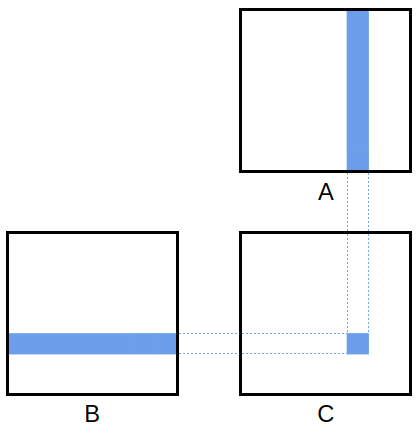
\includegraphics[width=0.5\textwidth]{1.png}
	\caption{Wykorzystanie pamięci globalnej}
\end{figure}

\begin{figure}[h]
	\centering
	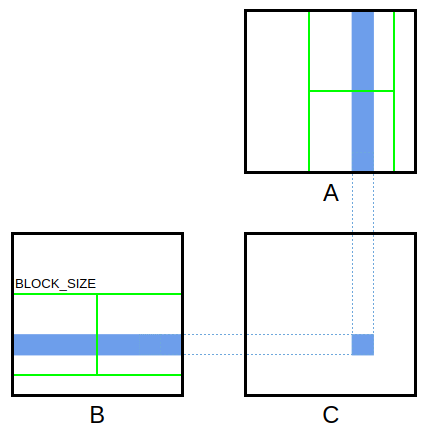
\includegraphics[width=0.5\textwidth]{2.png}
	\caption{Wykorzystanie pamięci podręcznej, dostęp niełączony}
\end{figure}

W przypadku pamięci globalnej każdy wątek odczytuje jeden wiersz macierzy A i jedną
kolumnę macierzy B, a następnie oblicza odpowiadający element macierzy C. Wszystkie
dane odczytywane są bezpośrednio z pamięci globalnej, co powoduje bardzo dużą liczbę odwołań
do pamięci globalnej.\\
W drugim przypadku, dla pamięci współdzielonej bloku wątków, każdy blok oblicza macierz
będącą częścią macierzy wynikowej C o rozmiarze równym rozmiarowi bloku. Każdy wątek
jest wówczas odpowiedzialny za obliczenie jednego elementu takiego wycinka macierzy.
W taki sposób znacząco ograniczamy ilość dostępów do pamięci globalnej, ponieważ macierze
A i B są odczytywane tylko $\frac{n}{BLOCK\_SIZE}$ razy, gdzie $n$ to wielkość instancji a
$BLOCK\_SIZE$ to wielokść bloku.

\section{Analiza wyników eksperymentu pomiarowego}
\subsection{Miary efektywności}
\subsubsection*{Prędkość obliczeń}
\begin{equation}
	\frac{ZL}{C} = \frac{2 * n^3}{C}
\end{equation}
gdzie $ZL$ to złożoność obliczeniowa, $C$ to czas a $n$ to rozmiar instancji.

\subsubsection*{Przyspieszenie w stosunku do IKJ}
\begin{equation}
	\frac{C\_IKJ}{CPR}
\end{equation}
gdzie $C\_IKJ$ to czas przetwarzania IKJ a $CPR$ to czas przetwarzania równoległego.

\subsubsection*{Przyspieszenie w funkcji wielkości instancji}
\begin{equation}
	\frac{CPI}{CP 128}
\end{equation}
gdzie $CPI$ to czas przetwarzania dla instancji a $CPI 128$ to czas przetwarzania dla
instancji o rozmiarze 128, będący naszym punktem odniesienia - obliczamy przyspieszenie
w stosunku do przetwarzania instancji o rozmiarze 128.

\subsubsection*{Miara stopnia łączenia dostępów do pamięci}
Jest to miara obliczana w następujący sposób: dla każdebo bloku pobierane
będą dwie macierze ($n^2$), dodajemy do tego $n^2$ zapisów do pamięci globalnej
i dzielimy przez sumę transkacji między pamięcią a multiprocesorem (odczytane
z wyników z programu Visual Profiler).\\

\subsubsection*{Zajętość procesora}
Wyliczana za pomocą kalkulatora zajętości SM miara - dla bloków o rozmiarze
8x8 osiąga $50\%$, zaś dla bloków o rozmiarze 16x16 osiąga $100\%$, czego można
się było spodziewać. Pokazuje to, że pełnię możliwości tej karty wykorzystujemy
wtedy, gdy bloki mają rozmiar 16x16.

\subsubsection*{CGMA - stosunek operacji do dostępów do pamięci}
Jest to miara instensywności obliczeń. Zakładamy, że do obliczenia jednego elementu
wynikowego potrzebujemy n danych z wiersza macierzy, n danych z kolumny macierzy
oraz 1 operację zapisu do pamięci globalnej.\\
Warto zauważyć, że dla współdzielonej pamięci bloku wątków CGMA będzie bliski 1,
ponieważ pomijamy operacje pobierania danych z pamięci globalnej do lokalnej.

gdzie $n$ to wielkość instancji.

\subsubsection*{GLD\_EFFICIENCY}
Jest to miara efektywności pobierania danych z pamięci globalnej obliczana w sposób
następujący:
\begin{equation}
	\frac{gld\_reques}{gld\_total / (2*SM)}
\end{equation}
gdzie $SM$ to liczba multiprocesorów.

\subsubsection*{GST\_EFFICIENCY}
Jest to miara efektywności zapisu danych w pamięci globalnej.
Oblicza się ją analogicznie
do GLD\_EFFICIENCY.
\begin{equation}
	\frac{gst\_reques}{(gst\_32 + gst\_64 + gst\_128) / (2*SM)}
\end{equation}
gdzie $SM$ to liczba multiprocesorów.

\subsection{Wyniki pomiarów}

\begin{table}


\end{table}

\begin{center}
	\begin{tabular}{ |c|c|c|c|c|c|c|c|c|c|c| }
		\hline
		V & BS & INST & GFLOPS & vs IKJ & $\Delta A$ & CMGA & JOIN & \% &  GLD\_E & GST\_E \\ \hline
		G\_L   & 8  & 128  & 25,32073626 & 12,0739 & 1,0000    & 0,0039 & 733,8826   & 50\%  & 5184     & 141208  \\ \hline
		      &    & 256  & 30,63327366 & 2,7388  & 6,6126    & 0,0019 & 1512,4980  & 50\%  & 10368    & 10904   \\ \hline
		      &    & 512  & 26,32677471 & 2,6480  & 61,5543   & 0,0010 & 3045,1146  & 50\%  & 20736    & 591     \\ \hline
		      &    & 864  & 22,22919876 & 2,4298  & 350,3191  & 0,0006 & 5162,9016  & 50\%  & 34992    & 59      \\ \hline
		      &    & 1024 & 24,66069324 & 5,8681  & 525,7037  & 0,0005 & 6120,9971  & 50\%  & 41472    & 35      \\ \hline
		      & 16 & 128  & 33,95345298 & 16,1903 & 1,0000    & 0,0039 & 245,8109   & 100\% & 1728     & 282894  \\ \hline
		      &    & 256  & 32,58490086 & 2,9133  & 8,3360    & 0,0019 & 552,7462   & 100\% & 3456     & 17551   \\ \hline
		      &    & 512  & 34,41340787 & 3,4614  & 63,1446   & 0,0010 & 1136,8067  & 100\% & 6912     & 1141    \\ \hline
		      &    & 864  & 32,75306701 & 3,5801  & 318,8183  & 0,0006 & 1930,8138  & 100\% & 11664    & 133     \\ \hline
		      &    & 1024 & 29,89612411 & 7,1139  & 581,4857  & 0,0005 & 2286,2996  & 100\% & 13824    & 63      \\ \hline
		G\_NL  & 8  & 128  & 10,11192223 & 4,8217  & 1,0000    & 0,0039 & 242,4433   & 50\%  & 3888     & 77004   \\ \hline
		      &    & 256  & 9,662213325 & 0,8639  & 8,3723    & 0,0019 & 501,8743   & 50\%  & 7776     & 4603    \\ \hline
		      &    & 512  & 6,010390691 & 0,6045  & 107,6740  & 0,0010 & 1012,7101  & 50\%  & 15552    & 181     \\ \hline
		      &    & 864  & 6,303300587 & 0,6890  & 493,3749  & 0,0006 & 1718,6194  & 50\%  & 26244    & 23      \\ \hline
		      &    & 1024 & 4,254822746 & 1,0124  & 1216,8084 & 0,0005 & 2037,9817  & 50\%  & 31104    & 8       \\ \hline
		      & 16 & 128  & 5,148311945 & 2,4549  & 1,0000    & 0,0039 & 29,1321    & 100\% & 3672     & 41510   \\ \hline
		      &    & 256  & 5,148414636 & 0,4603  & 7,9998    & 0,0019 & 65,2732    & 100\% & 7344     & 2595    \\ \hline
		      &    & 512  & 3,569637799 & 0,3590  & 92,3040   & 0,0010 & 133,9956   & 100\% & 14688    & 112     \\ \hline
		      &    & 864  & 3,316741109 & 0,3625  & 477,3804  & 0,0006 & 227,4108   & 100\% & 24786    & 13      \\ \hline
		      &    & 1024 & 2,167744905 & 0,5158  & 1215,9806 & 0,0005 & 269,2327   & 100\% & 29376    & 4       \\ \hline
		S\_L   & 8  & 128  & 33,09585582 & 15,7813 & 1,0000    & 1      & 3879,0936  & 50\%  & 864      & 1112210 \\ \hline
		      &    & 256  & 38,81404571 & 3,4702  & 6,8214    & 1      & 8493,2578  & 50\%  & 1728     & 82978   \\ \hline
		      &    & 512  & 39,20490797 & 3,9433  & 54,0273   & 1      & 17661,6646 & 50\%  & 3456     & 5254    \\ \hline
		      &    & 864  & 23,68074399 & 2,5885  & 429,8229  & 1      & 25701,0879 & 50\%  & 6912     & 330     \\ \hline
		      &    & 1024 & 65,60469794 & 15,6108 & 258,2906  & 1      & 42639,0980 & 50\%  & 5832     & 652     \\ \hline
		      & 16 & 128  & 17,17252759 & 8,1885  & 1,0000    & 1      & 2352,7619  & 100\% & 0        & 2155375 \\ \hline
		      &    & 256  & 20,78304377 & 1,8581  & 6,6102    & 1      & 6582,7043  & 100\% & 0        & 170279  \\ \hline
		      &    & 512  & 21,7859839  & 2,1913  & 50,4472   & 1      & 15496,4703 & 100\% & 0        & 11433   \\ \hline
		      &    & 864  & 21,82694331 & 2,3858  & 241,9650  & 1      & 27996,8000 & 100\% & 0        & 1426    \\ \hline
		      &    & 1024 & 21,80557117 & 5,1887  & 403,2150  & 1      & 33641,2658 & 100\% & 0        & 724     \\ \hline
		S\_NL  & 8  & 128  & 31,95027271 & 15,2351 & 1,0000    & 1      & 1429,1397  & 50\%  & 540      & 1726347 \\ \hline
		      &    & 256  & 38,67665172 & 3,4580  & 6,6087    & 1      & 3247,4221  & 50\%  & 1080     & 132073  \\ \hline
		      &    & 512  & 39,13595265 & 3,9364  & 52,2491   & 1      & 6899,0877  & 50\%  & 2160     & 8390    \\ \hline
		      &    & 864  & 39,36259325 & 4,3026  & 249,6331  & 1      & 11969,1021 & 50\%  & 3645     & 1041    \\ \hline
		      &    & 1024 & 35,79431614 & 8,5174  & 457,0150  & 1      & 14265,8722 & 50\%  & 4320     & 487     \\ \hline
		      & 16 & 128  & 16,64049767 & 7,9348  & 1,0000    & 1      & 297,6386   & 100\% & 229,5    & 2118706 \\ \hline
		      &    & 256  & 20,38662765 & 1,8227  & 6,5300    & 1      & 810,5569   & 100\% & 459      & 164427  \\ \hline
		      &    & 512  & 21,71864653 & 2,1845  & 49,0358   & 1      & 1871,3958  & 100\% & 918      & 10961   \\ \hline
		      &    & 864  & 21,81985743 & 2,3851  & 234,5448  & 1      & 3348,4545  & 100\% & 1549,125 & 1358    \\ \hline
		      &    & 1024 & 21,79336548 & 5,1858  & 390,9417  & 1      & 4014,0147  & 100\% & 1836     & 688     \\ \hline
	\end{tabular}
	\captionof{table}{Miary efektywności dla 6 pętli, przetwarzanie równolegle}
\end{center}

\section{Wnioski}
Po przeanalizowaniu wyników


\end{document}